\documentclass[citation\_needed]{subfiles}
\begin{document}

Le réseau présenté par \citet{lample2016neural} est une variante enrichie de l'approche définie par \citet{huang2015bidirectional}, où la sortie d'un LSTM est donnée à un CRF afin que ce dernier prédise la séquence. L'intérêt de l'ajout d'un CRF est que ce dernier, contrairement au LSTM, intègre des constraintes structurelles sur l'espace de sortie, un LSTM prédisant "indépendamment" une sortie pour chaque élément de la séquence, dont une vision d'ensemble est disponible dans la figure\ \ref{fig:lstm-CRF}. L'intérêt du réseau de \citet{lample2016neural} réside dans les ajouts qu'il fait à ce modèle : notamment une couche de sélection (dropout) ainsi qu'une représentation du token calculée au niveau des caractères. Cette représentation est faite via un LSTM bidirectionnel, cela permet de capturer des informations morphologiques en termes de préfixes et suffixes du token. La représentation finale d'un token est donc la concaténation des trois représentations suivantes : celle de sa forme de surface, celle de ses préfixes et celle de ses suffixes comme illustré sur la figure\ \ref{fig:lstm-CRF}. Cela est comparable à ajouter une analyse morphologique à chaque token.

\begin{figure}[ht!]
\begin{minipage}{0.49\linewidth}
    \centering
    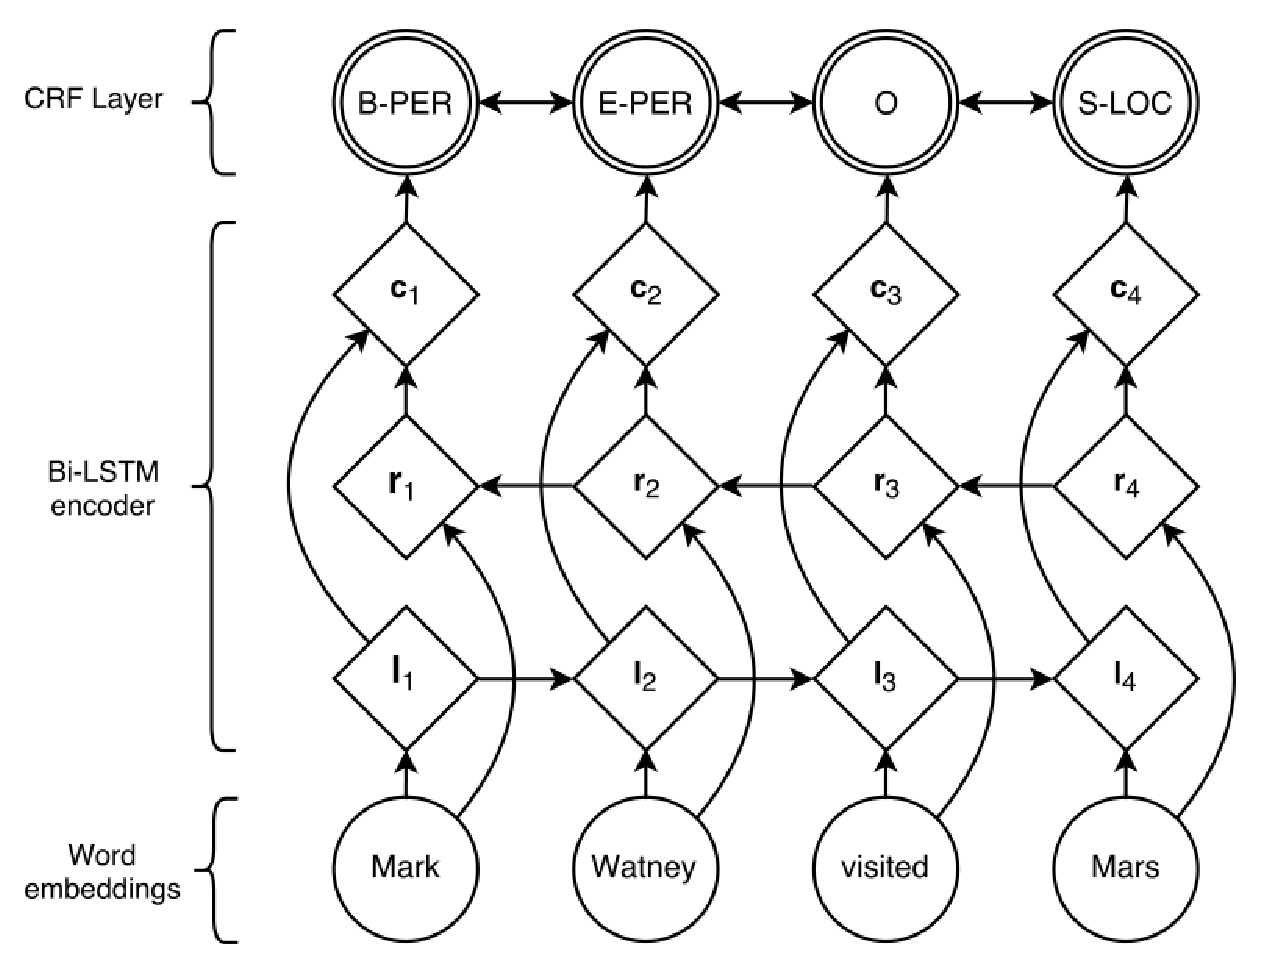
\includegraphics[scale=0.35]{images/LSTM/LSTM-CRF}
\end{minipage}
\begin{minipage}{0.49\linewidth}
    \centering
    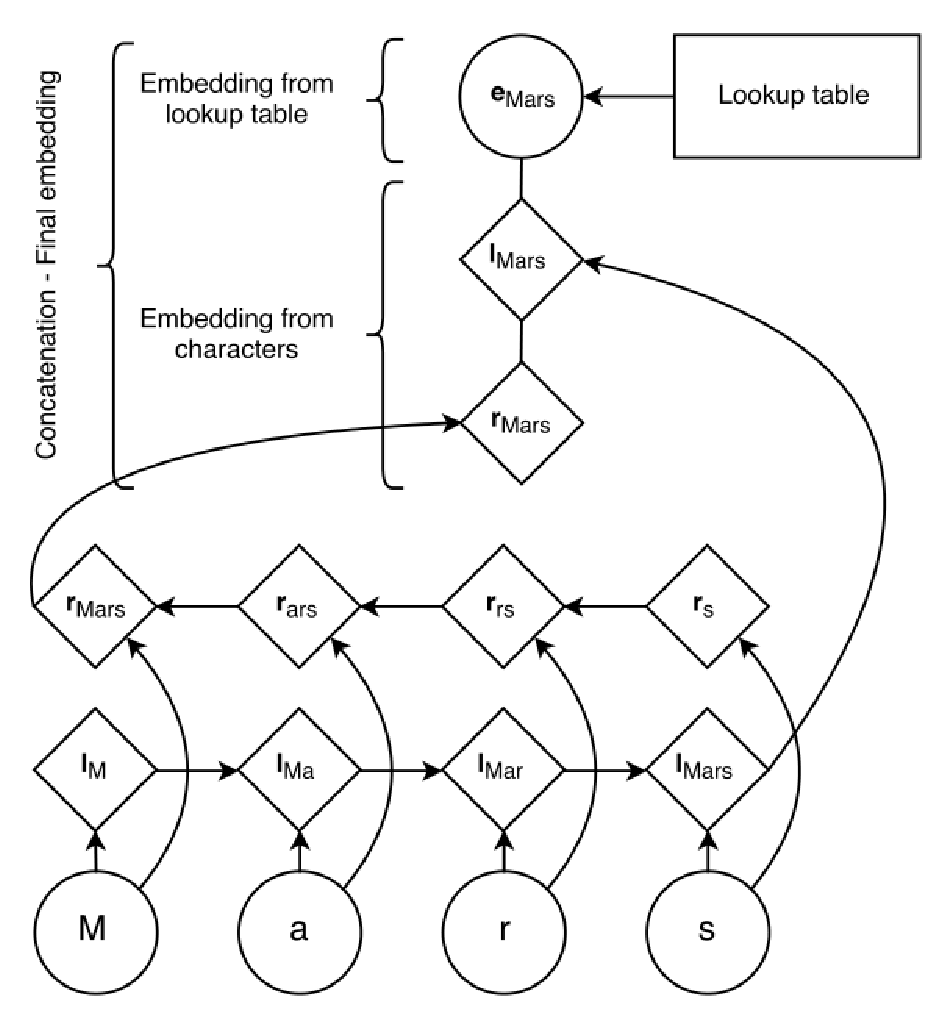
\includegraphics[scale=0.4]{images/LSTM/LSTM-char}
\end{minipage}
\caption{À gauche : le modèle LSTM-CRF pour une phrase. À droite : Le réseau LSTM pour un token}
\label{fig:lstm-CRF}
\end{figure}

\end{document}